\documentclass[letterpaper,12pt]{article}
\usepackage{tabularx} % extra features for tabular environment
\usepackage{amsmath}  % improve math presentation
\usepackage{graphicx} % takes care of graphic including machinery
\usepackage[margin=1in,letterpaper]{geometry} % decreases margins
\usepackage{cite} % takes care of citations
\usepackage[final]{hyperref} % adds hyper links inside the generated pdf file
\hypersetup{
	colorlinks=true,       % false: boxed links; true: colored links
	linkcolor=blue,        % color of internal links
	citecolor=blue,        % color of links to bibliography
	filecolor=magenta,     % color of file links
	urlcolor=blue         
}
\usepackage{blindtext}

\usepackage{listings}
\lstset{
  basicstyle=\ttfamily,
  columns=fullflexible,
  frame=single,
  breaklines=true,
  postbreak=\mbox{\textcolor{red}{$\hookrightarrow$}\space},
}

\renewcommand{\abstractname}{Executive Summary}


%++++++++++++++++++++++++++++++++++++++++

\setlength{\parindent}{4em}
\setlength{\parskip}{1em}
\begin{document}

\title{CSCI-539 Project 3: Testing the Effects of Pre-filtering on the Learning to Rank Pipeline}
\author{Jeffery Russell, Badah Shin}

\date{\today}
\maketitle

\begin{abstract}
In this project, we examine the effect that the top-k selection algorithm has on the Learning to Rank (LTR) pipeline.
All experiments conduct using PyTerrier and both the Vaswani and the 2019 Trec Deep Learning Dataset.
After comparing Normalized Discount Cumulative Gain(NDCG), Mean Average Precision(MAP), and execution time against two top-k selection algorithms, we made a few conclusions. First, we noted that with a significantly large value for K, the performance of the LTR pipelines would converge regardless of what top-k selection model was used. Second, we demonstrated that K's value would have a linear relationship with the time it takes to rank each query with an LTR pipeline.

\begin{description}
\item[Keywords]
Information Retrieval, Learning to Rank
\end{description}

\end{abstract}
\maketitle

\section{Experiment Overview and Design}

Terrier is an open-source search engine created by the Department of Computing Science at the University of Glasgow for research and experimentation in text retrieval. The core software is written in java and offers a python API to the core software. The source for both core and python API can be accessed in the following link: \url{https://github.com/terrier-org}.

We used the python API because we were more familiar with python. It allowed us to create a jupyter notebook for quick experimentation and easy loading for graphs and tables.
We used libraries such as NumPy for matrix and/or vector calculations, pandas for tables, matplotlib for graph visualization, and sklearn for the machine learning algorithm. 

Learning to rank in production uses two ranking algorithms to rank documents, as shown in figure \ref{fig:ltr_pipeline}. 
The first ranking algorithm is a traditional ranking model to generate a ranked list-- such as TF-IDF, BM25, and PL2.
The second-ranking algorithm combines use features of a document to rank the algorithm.
These features could be things from TF-IDF, BM25, or metadata like page rank, last update time, etc.
The learning model can be trained with the training data that consists of queries and documents.

\begin{figure*}[h!]
    \centering  % this centers the graphic on the page
    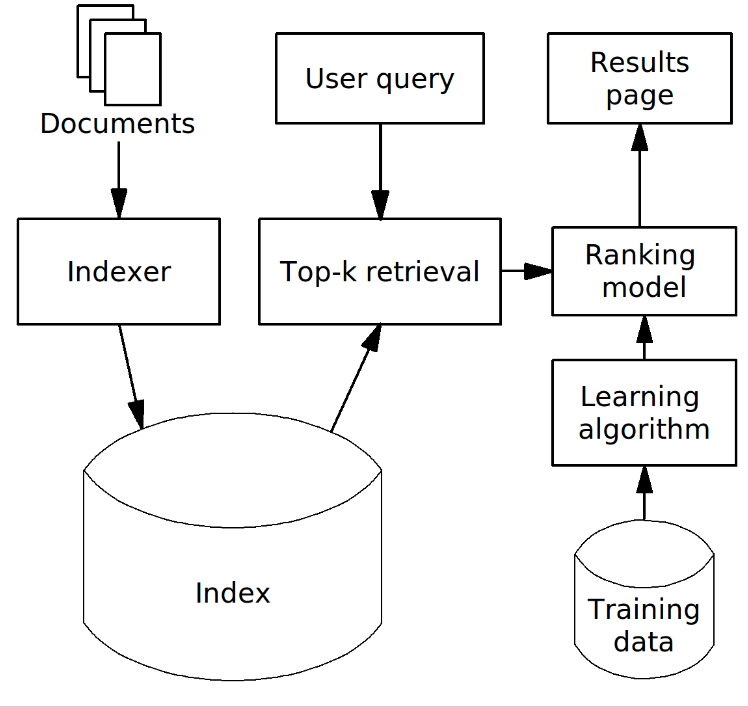
\includegraphics[width=.80\textwidth]{model.png} % graphic has a width of 80% of the page
    \caption{A diagram of a machine learning search engine} % text to display with figure
    \label{fig:ltr_pipeline} % label for you to cite the figure with
\end{figure*}


We were interested in the fact that in a learn-to-rank (LTR) algorithms, not every single document in the corpus gets ranked upon retrieval by the ML model.
Instead, an initial ranking function gets used to select the top k documents that are then run through the learning algorithm.
This pre-processing step gets done since the features and algorithms used in the ML model are much more computationally expensive to run than the pre-processing step.
After we receive our top k documents, a more computationally expensive machine learning algorithm is used to re-rank the documents.
This experiment aims to isolate the top-k retrieval step and figure out how the selection of K and the retrieval model affects end performance in terms of accuracy and efficiency.

\section{Collections Used}

In this project, we used two datasets: Vaswani and Trec Deep Learning.
In Pyterrier, the name of the dataset can be browsed in the DATASET MAP dictionary under the datasets.py file.
The content of the data can be accessed with methods inside ‘dataset’ such as get-index(), get-topics(), get-qrels(), and get-corpus(). 
These functions are not always reliable.
If the program runs on a Unix system, the dataset is saved in the file path “.pyterrier/corpora/”. 
The corpus is in the “corpus” folder saved as a .trec file.


\subsection{Collection 1: vaswani}
Vaswani dataset is known as the Vaswani and Cameron NPL test collection.
It is the default dataset for the pyterrier. The source code dataset includes easy access to the corpus, topics, qrels, and index. 
The total number of documents is 11429, and the total number of queries is 93. 

The following are sample queries from the vaswani dataset:

\begin{lstlisting}[frame=single]  
Query 1: qid 1
MEASUREMENT OF DIELECTRIC CONSTANT OF LIQUIDS BY THE USE OF MICROWAVE TECHNIQUES
\end{lstlisting}

\begin{lstlisting}[frame=single]  
Query 2: qid 2
MATHEMATICAL ANALYSIS AND DESIGN DETAILS OF WAVEGUIDE FED MICROWAVE RADIATIONS
\end{lstlisting}

\begin{lstlisting}[frame=single]  
Query 3: qid 3
USE OF DIGITAL COMPUTERS IN THE DESIGN OF BAND PASS FILTERS HAVING GIVEN PHASE AND ATTENUATION CHARACTERISTICS
\end{lstlisting}

The following are sample document bodies from the vaswani dataset:

\begin{lstlisting}[frame=single]  
Document 1: doc no 1
compact memories have flexible capacities  a digital data storage
system with capacity up to bits and random and or sequential access
is described
\end{lstlisting}

\begin{lstlisting}[frame=single]  
Document 2: doc no 2
an electronic analogue computer for solving systems of linear equations
mathematical derivation of the operating principle and stability
conditions for a computer consisting of amplifiers
\end{lstlisting}

\begin{lstlisting}[frame=single]  
Document 3: doc no 3
electronic coordinate transformer  circuit details are given for
the construction of an electronic calculating unit which enables
the polar coordinates of a vector modulus and cosine or sine of the
argument to be derived from those of a rectangular system of axes
\end{lstlisting}



\subsection{Collection 2: trec-deep-learning-docs}

Trec-deep-learning-docs dataset is known as the MS-MARCO dataset from TREC Deep Learning Track. 
The version we used was the 2019 version \cite{trec-deep-learning}.
It is designed to be a large dataset for training with deep learning models. The total number of documents is 3,213,835, and the total number of queries is 200.
The index needs to be generated, and the get-index() is broken, so we used the following line:

\begin{lstlisting}[frame=single]  
indexref = indexer.index(dataset.get_corpus())
\end{lstlisting}
The next following line retrieves the index from a saved file. 

\begin{lstlisting}[frame=single]  
indexref = pt.autoclass("org.terrier.querying.IndexRef").of(os.path.join(index_path, "data.properties"))
\end{lstlisting}


\begin{figure*}[h!]
    \centering  % this centers the graphic on the page
    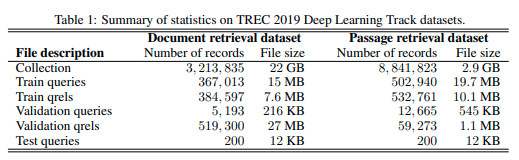
\includegraphics[width=1\textwidth]{table_trec.png} % graphic has a width of 80% of the page
    \caption{TREC 2019 Collection Summary, Table Included from Paper: \cite{trec-deep-learning}}% text to display with figure
    \label{fig:trec_table} % label for you to cite the figure with
\end{figure*}

The following are sample queries from the trec deep learning dataset:

\begin{lstlisting}[frame=single]  
Query 1: qid 1108939
what slows down the flow of blood
\end{lstlisting}

\begin{lstlisting}[frame=single]  
Query 2: qid 1112389
what is the county for grand rapids mn
\end{lstlisting}

\begin{lstlisting}[frame=single]  
Query 3: qid 792752
what is ruclip
\end{lstlisting}

The following are sample documents from the Trec deep learning dataset.
Note: that "..." means that the entire document was not included because it was too long.

\begin{lstlisting}[frame=single]  
Document 1: doc no D1555982
https://answers.yahoo.com/question/index?qid=20071007114826AAwCFvR
The hot glowing surfaces of stars emit energy in the form of electromagnetic radiation.?
Science & Mathematics Physics
...
\end{lstlisting}

\begin{lstlisting}[frame=single]  
Document 2: doc no D301595
http://childparenting.about.com/od/physicalemotionalgrowth/tp/Child-Development-Your-Eight-Year-Old-Child.htm
Developmental Milestones and Your 8-Year-Old Child
...
\end{lstlisting}

\begin{lstlisting}[frame=single]  
Document 3: doc no D1359209
http://visihow.com/Check_for_Lice_Nits
Check for Lice Nits
Check for Lice Nits
...
\end{lstlisting}

The biggest thing to note with these documents are that the document lengths are much larger than that of the Vaswani dataset. 


\section{Methodology}

In our project, we aim to isolate the effect of the top-k retrieval so that we can make modifications to it and examine the results.
To do so, we created a generic pipeline outlined in figure \ref{fig:gen-pipeline}.
The first step in the pipeline is to download and index our corpus -- in our case Vaswani or Trec Deep Learning.

\begin{figure*}[h!]
    \centering  % this centers the graphic on the page
    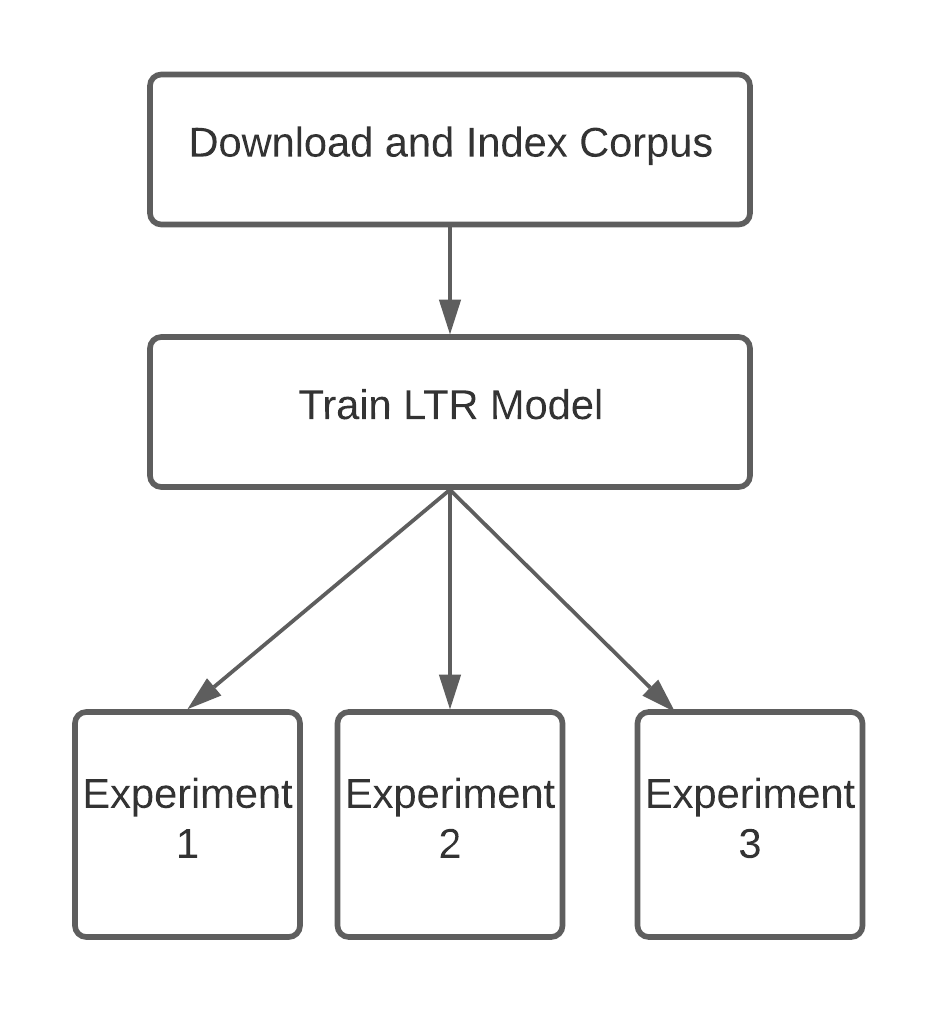
\includegraphics[width=.6\textwidth]{method.png} % graphic has a width of 80% of the page
    \caption{Data Flow for Experimentation} % text to display with figure
    \label{fig:gen-pipeline} % label for you to cite the figure with
\end{figure*}


The second phase in the pipeline is to train an LTR model. For the sake of simplicity, we are training a Random Forest Regressor using Sklearn \cite{scikit-learn}.
The features used the random forest regression model are as follows: "WMODEL:TF-IDF", "WMODEL:PL2", "WMODEL:DPH", "WMODEL:BM25".
For example, the "WMODEL:TF-IDF" feature is simply the TF-IDF score of a document compared to the query.

For each dataset that we test with, we only create a single ML model.
This singular model is then used in all subsequent queries to aid inconsistency in our results.

\section{Results and Discussion}
% 3-4 pages

This section goes over the different experiments that we ran and the resulting performance.

\subsection{Experiment 1: Effect on NDCG}
\label{sec:ex1}

We experimented on the effect that varying K had on Normalized Discount Cumulative Gain (NDCG).
We also wanted to see how varying top k selection algorithms compare to each other for NDCG.
To do this, we instantiated each retrieval pipeline by using the baseline algorithm and adding a pipe operator that only selects the top K results and then feeds those results into the learning to rank model.
If we test the baseline performance, we still add the top k filter, but we do not pass it into a second-ranking model.
The Vaswani dataset results are shown in figure \ref{fig:ex_ndcg_vaswani}, and the results on the Trec deep learning dataset are shown in figure \ref{fig:ex_ndcg_deep}.

\begin{figure*}[h!]
    \centering  % this centers the graphic on the page
    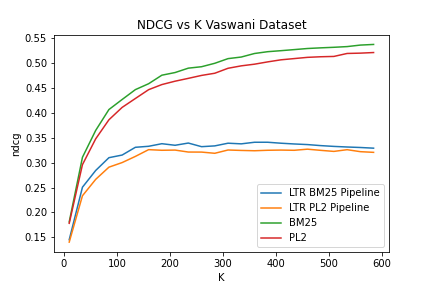
\includegraphics[width=.81\textwidth]{NDCG-vs-K-Vaswani-Dataset.png} % graphic has a width of 80% of the page
    \caption{Effect of K on NDCG on Various Ranking Pipelines Vaswani Dataset} % text to display with figure
    \label{fig:ex_ndcg_vaswani} % label for you to cite the figure with
\end{figure*}

\begin{figure*}[h!]
    \centering  % this centers the graphic on the page
    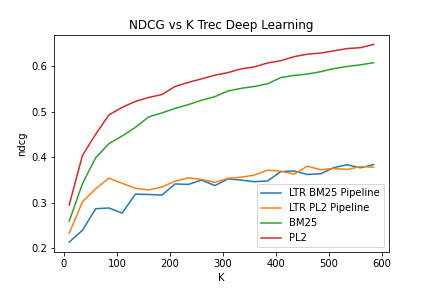
\includegraphics[width=.81\textwidth]{NDCG-vs-K-Trec-Deep-Learning.png} % graphic has a width of 80% of the page
    \caption{Effect of K on NDCG on Various Ranking Pipelines Trec Deep Learning Dataset} % text to display with figure
    \label{fig:ex_ndcg_deep} % label for you to cite the figure with
\end{figure*}

As shown in the Vaswani dataset results in figure \ref{fig:ex_ndcg_vaswani}, the results for NDCG appear to increase for K monotonically, and that the results for the BM25 algorithms are slightly better than the BM25 algorithms.
However, Vaswani's results are to be taken with a grain of salt due to their small dataset size.
The results for the larger deep learning set in figure \ref{fig:ex_ndcg_deep} tell a slightly different story from the Vaswani dataset.
Rather than differ by some fixed amount regardless of K, the two LTR pipelines converged as K's value increased.
This convergence suggests that if you select a large enough K, your performance is close to identical regardless of what reasonable top K selection algorithm you use.

\subsection{Experiment 2: Effect on MAP}

Similar to the experiment outlined in section \ref{sec:ex1}, this experiment examines the difference between varying K, the top-k selection model, and Mean Average Precision (MAP).
Figure \ref{fig:ex_map_vaswani} show the results on the Vaswani dataset and figure \ref{fig:ex_map_deep} illustrates the results on the Trec deep learning dataset.


\begin{figure*}[h!]
    \centering  % this centers the graphic on the page
    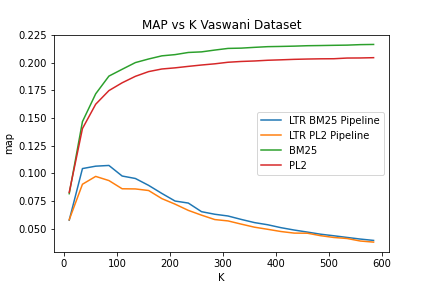
\includegraphics[width=.81\textwidth]{MAP-vs-K-Vaswani-Dataset.png} % graphic has a width of 80% of the page
    \caption{Effect of K on MAP on Various Ranking Pipelines Vaswani Dataset} % text to display with figure
    \label{fig:ex_map_vaswani} % label for you to cite the figure with
\end{figure*}

\begin{figure*}[h!]
    \centering  % this centers the graphic on the page
    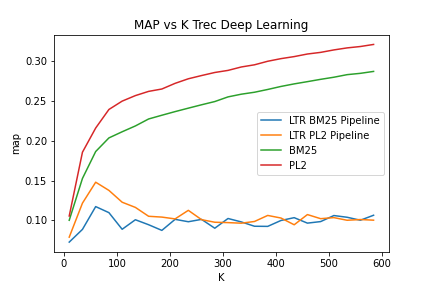
\includegraphics[width=.81\textwidth]{MAP-vs-K-Trec-Deep-Learning.png} % graphic has a width of 80% of the page
    \caption{Effect of K on MAP on Various Ranking Pipelines Trec Deep Learning Dataset} % text to display with figure
    \label{fig:ex_map_deep} % label for you to cite the figure with
\end{figure*}

Similar to the prior section, the results of the Vaswani dataset and the Deep learning dataset vary.
In the Vaswani dataset, the BM25 LTR pipeline always had a slight advantage over the PL2 LTR pipeline, where in the Trec Deep Learning dataset, the two LTR pipelines ended up converging.
This supports the conclusion made in the prior section that having a sufficiently large enough K will result in the pipelines' answers to converge.
Additionally, we can see that for both MAP and NDCG, the results with small K show different results between different pipelines.


\subsection{Experiment 3: Effect on Execution Time}

In this experiment, we aim to quantify how varying K affects how fast retrieval will be.
It is expected that as we increase K, our execution time will increase because our ML ranking algorithm will have to re-rank more documents.
To measure this, we will be using Python's datetime library, where we measure the time it takes to evaluate the entire test collection against our labeled data using our LTR pipeline.
Although this does not measure the time it takes to rank a single query, K's relationship is still applicable.

Since we are taking empirically measuring performance on a computer, some variations and spikes in the data are expected.
To remove some of this jitter, for each measurement, we took the average of N trials. For the Vaswani dataset in figure \ref{fig:ex_time_vaswani}, we did ten trials for each point.
For the Trec deep learning dataset in figure \ref{fig:ex_time_ms}, we took three samples.
This reduction in the amount of points sampled is merely to accommodate that running a trial of this scale on a dataset as large as the Deep Learning set would take an egregious amount of time. 

\begin{figure*}[h!]
    \centering  % this centers the graphic on the page
    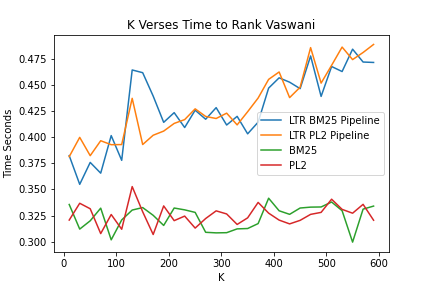
\includegraphics[width=.81\textwidth]{K-Verses-Time-to-Rank-Vaswani.png} % graphic has a width of 80% of the page
    \caption{Execution Time of Different Ranking Pipelines on Vaswani Dataset} % text to display with figure
    \label{fig:ex_time_vaswani} % label for you to cite the figure with
\end{figure*}


In figure \ref{fig:ex_time_vaswani}, the LTR pipeline's performance is shown along with the baseline performance of running the ranking and then filtering using only the initial ranking algorithm.
As to be expected, using only BM25 or PL2, the value of K is not significant since these algorithms rank the entire corpus, and then filtering for the top K is a trivial task.
The Results for both the BM25 pipeline and PL2 pipelines appeared to be approximately the same using the small Vaswani corpus.


Figure \ref{fig:ex_time_ms} illustrates the results of varying K on the execution time of evaluating the Trec Deep learning dataset.
Similar to the Vaswani results, as we increased the value of K, the execution time increased.
With figure \ref{fig:ex_time_ms}, it is also apparent that there is a difference in execution time between using BM25 and PL2.

With the Vaswani results in figure \ref{fig:ex_time_vaswani}, both algorithms appeared to be equally fast. In figure \ref{fig:ex_time_ms}, BM25 is always faster than PL2 by a linear factor.

\begin{figure*}[h!]
    \centering  % this centers the graphic on the page
    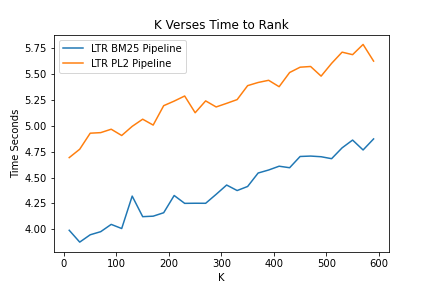
\includegraphics[width=.81\textwidth]{K-Verses-Time-to-Rank.png} % graphic has a width of 80% of the page
    \caption{Execution Time of Different Ranking Pipelines on Trec Deep Learning} % text to display with figure
    \label{fig:ex_time_ms} % label for you to cite the figure with
\end{figure*}


\section{Conclusion}

Running empirical studies is essential in CS when determining optimal hyperparameter to use in a system.
Although it is easy to pick the default values given by a system, it is essential to run experiments and find the optimal parameters to use in your environment.
This paper explored two critical parameters when implementing LTR in practice: choice of k and top-k selection algorithm.
We found that there was a sweet spot when selecting a value for K.
If we choose a value too high, it is computationally expensive; however, if we choose a value too low, the average performance in terms of MAP and NDCG will suffer.
Additionally, we found that the LTR ranking results will converge regardless of what initial top-k-selection algorithm you use, granted that your value for K is sufficiently large.

\bibliographystyle{plain}
\bibliography{ref}

\end{document}

